\documentclass[conference]{IEEEtran}
\interdisplaylinepenalty=2500

\usepackage{array}
\usepackage{graphicx}
\usepackage{epsf}
\usepackage{float}
\usepackage{stfloats}
\usepackage[font=footnotesize]{caption}
\usepackage[font=footnotesize]{subcaption}
\usepackage{cite}
\usepackage{picinpar}
\usepackage{siunitx}

\usepackage{amsmath, nccmath}
\usepackage{url}
\usepackage{flushend}
\usepackage{colortbl}
\usepackage{soul}
\usepackage{multirow}
\usepackage{pifont}
\usepackage{color}
\usepackage{alltt}
\usepackage[hidelinks]{hyperref}
\usepackage{enumerate}
\usepackage{siunitx}
\usepackage{breakurl}
\usepackage{epstopdf}
\usepackage{pbox}


\usepackage{booktabs}
\usepackage{wrapfig}

\graphicspath{{../}}

\usepackage{placeins}
\usepackage{latexsym}
\usepackage{amssymb}
\usepackage{xifthen}
\usepackage{balance}
\usepackage{multicol}
\renewcommand{\arraystretch}{1.2}




\newenvironment{conditions}
  {\par\vspace{\abovedisplayskip}\noindent\begin{tabular}{>{$}l<{$} @{${}-{}$} l}}
  {\end{tabular}\par\vspace{\belowdisplayskip}}


\ifCLASSINFOpdf

\else
 
\fi


\hyphenation{op-tical net-works semi-conduc-tor}


\begin{document}

\title{Analysis and DSP Implementation of Multisampled Three-Phase Current Controllers}

\author{\IEEEauthorblockN{1\textsuperscript{st} Ivan Petric}
\IEEEauthorblockA{\textit{Depart. of Information Engineering} \\
\textit{University of Padova}\\
Padova, Italy \\
petric@dei.unipd.it}
\and
\IEEEauthorblockN{2\textsuperscript{nd} Ruzica Cvetanovic}
\IEEEauthorblockA{\textit{Dept. of Power Engineering} \\
\textit{University of Belgrade}\\
Belgrade, Serbia \\
ruzica996@gmail.com}
\and
\IEEEauthorblockN{3\textsuperscript{rd} Paolo Mattavelli}
\IEEEauthorblockA{\textit{Dept. of Management and Engineering} \\
\textit{University of Padova}\\
Vicenza, Italy \\
paolo.mattavelli@unipd.it}
\and
\IEEEauthorblockN{4\textsuperscript{th} Simone Buso}
\IEEEauthorblockA{\textit{Depart. of Information Engineering} \\
\textit{University of Padova}\\
Padova, Italy \\
simone.buso@dei.unipd.it}
}


% make the title area
\maketitle

\begin{abstract}
This paper presents a method for current control of three-phase systems, realized using the multisampled pulse-width modulator (MS-PWM). The feedback signal is highly oversampled and filtered to obtain its average value with high noise suppression. Independently, the control update rate is chosen to be higher than double the switching frequency, which reduces delays due to calculation and digital modulation. In this way, the proposed strategy offers improved dynamic response compared to standard double-update PWM, while offering a high quality feedback signal, robust to noise sampling and aliasing.
The analysis is verified using a standard digital signal processor TI f28379d and a Typhoon HIL 402 hardware-in-the-loop system that emulates an electric drive with a high-speed BLDC motor.
\end{abstract}

% Note that keywords are not normally used for peerreview papers.
\begin{IEEEkeywords}
Current control, Digital Pulse-Width Modulators (DPWM), Multisampled Pulse-Width Modulators (MS-PWM)
\end{IEEEkeywords}


\IEEEpeerreviewmaketitle

\section{Introduction}
\IEEEPARstart{F}{ield} oriented control (FOC) in electrical drives and voltage oriented control (VOC) in grid-connected converters is a well-established strategy for the control of high performance three-phase electrical systems \cite{holmes2012}. An essential part of this concept is the inner current control loop, which regulates the synchronous rotating frame (SRF) currents \cite{holmes2012}. The SRF controller must provide a decoupling function between $d$ and $q$ axis currents. This is particularly challenging for high-speed or high pole-pair electrical drives, which operate at very high output frequencies ~\cite{yim2009,Petric2021a}. 
Regarding controller structures, SRF proportional-integral (PI) controllers are most frequently used due to their simplicity and satisfactory performance for the majority of the industrial requirements ~\cite{yim2009,yepes2014}. However, their transient decoupling capability is rather limited, especially at high output frequencies \cite{lorenz2010}. Achieving a robust high-frequency operation and high bandwidths has driven the design of current controllers directly in discrete-time domain ~\cite{lorenz2010,vuksa2016,commentsHoffmann}. Belonging to this group are the dead-beat current controllers that offer a very fast transient response, but at the cost of considerable performance degradation in the presence of variable parameters and measurement errors, which is often the case in control of electric drives ~\cite{rovere2018,xu2019,Ito2021}. A more robust operation is achieved with the use of the discrete internal model controller (IMC) design ~\cite{lorenz2010,vuksa2016,commentsHoffmann}. This strategy has proven to offer high closed loop bandwidths at very high output frequencies ~\cite{commentsHoffmann,vuksa2016,Petric2021a}.

The demerit of digital control systems is the introduction of delays due to the analog-to-digital conversion (ADC), algorithm execution time, and digital pulse width modulation (DPWM) \cite{Buso2015}. These delays limit the achievable bandwidths and impair the decoupling function of SRF current controllers. 
In most state-of-the-art applications, double-sampled double-update (DS-DU-PWM) control strategy is used, where the feedback is sampled twice per PWM period, with acquisition instants being synchronized so that the average value is obtained \cite{Buso2015}. In industrial applications, the feedback signal is often strongly corrupted by various noise sources, which requires additional filtering \cite{vuksa2016}. Furthermore, sampling of the average value is compromised by system delays, which causes aliasing problems \cite{Buso2015}.
Improved error-free feedback acquisition is achieved by oversampling the signal and then averaging it over the PWM period using a moving average filter (MAF). In this way, the average value is obtained with additional high noise suppression \cite{vuksa2016,Petric2020}. The filtered signal is then decimated so that the control action is executed with the double-update rate. This kind of strategy, implemented in \cite{vuksa2016}, is here labeled as multi-sampled double-update (MS-DU-PWM) control. The MS-DU-PWM strategy results in a high quality feedback signal, however, it yields a negative impact on the system dynamics. Achieving high bandwidths with the one switching period averaging requires modification of the controller structure, to compensate the introduced phase lag \cite{vuksa2016}.
The delay-related limitations of digital control have inspired investigation of the multisampled PWM (MS-PWM) control, with purpose of enabling analog-like control bandwidths in digital systems. The multisampled multi-update (MS-MU-PWM) approach relies on acquiring the control variables and updating the modulating waveform multiple times per switching period ~\cite{corradini2018,corradini_analysis,rovere2018,Restrepo2019,Petric2020,Petric2021,Ito2021,He2021}. The concept of MS-MU-PWM digital control offers a significant delay reduction and is therefore a promising solution for breaking the bandwidth limitations of digital control systems \cite{corradini2018}. Besides the small-signal improvement, MS-MU-PWM also yields a lower response delay to large-signal perturbations as the modulating waveform can be updated multiple times per switching period \cite{Buso2016}. On the other hand, MS-MU-PWM introduces a set of nonlinearities, mainly due to the modulating waveform discontinuity as the switching ripple is introduced in the feedback ~\cite{corradini2018,Petric2021}. For this reason, most of the reported MS-MU-PWM methods include digital filtering, such as MAFs, to completely remove the switching ripple ~\cite{Restrepo2019,He2021}.

This paper analyzes the use of the digital MS-MU-PWM IMC-based current controller, suitable for implementation on standard DSP platforms. The main goal of the paper is to analyze the performance of MS-MU-PWM with one switching period averaging and to compare it with standardly used DS-DU-PWM and MS-DU-PWM methods. 
%The MS-PWM control strategy is analyzed for three different control loop organizations. The first one uses discrete IMC controller from \cite{vuksa2016}, with a moving average filter (MAF) in the feedback. This case is found to offer slightly improved dynamics compared to standard use of double-update with the same discrete IMC (without filter in feedback) ~\cite{lorenz2010,vuksa2016}, with significant improvement in jitter suppression. Due to added delays introduced by the MAF, the second case adds a derivative action to the controller structure, as in \cite{vuksa2016}. This case is given to demonstrate that MS-PWM can offer even better dynamics than reported in \cite{vuksa2016}. The final case implements MS-PWM based discrete IMC, without any filters in feedback. This case is expected to provide the best dynamics, using discrete IMC without derivative gain. The feedback quality is expected to worsen compared to cases with MAFs, hower, it still retains higher quality compared to double-update \cite{petric2020}. 
The target is to show that the MS-MU-PWM control with feedback averaging provides an improved dynamic performance compared to DS-DU-PWM, while offering a high quality feedback signal in the same manner as MS-DU-PWM.

This paper is organized as follows. Section II explains the multi-rate control structure and emphasizes benefits of MS-MU-PWM control. Subsequently, the discrete-time model of a three-phase $RL$ load is derived and used to obtain a model-based controller structure. Section III focuses on the implementation of multisampled feedback acquisition, filtering, and choice of the control update rate. In section IV, the controller gains are chosen for a suitable comparison between DS-DU, MS-DU, and MS-MU methods. The discrete-time modeling is verified using the sweep frequency response analysis. Section V provides experimental verification on the TI DSP f28379d and a hardware-in-the-loop emulation of a BLDC electric drive. The conclusions of the study are drawn in Section VI.
 
\section{Multi-rate control system}

\begin{figure*}[t!]
    \centerline{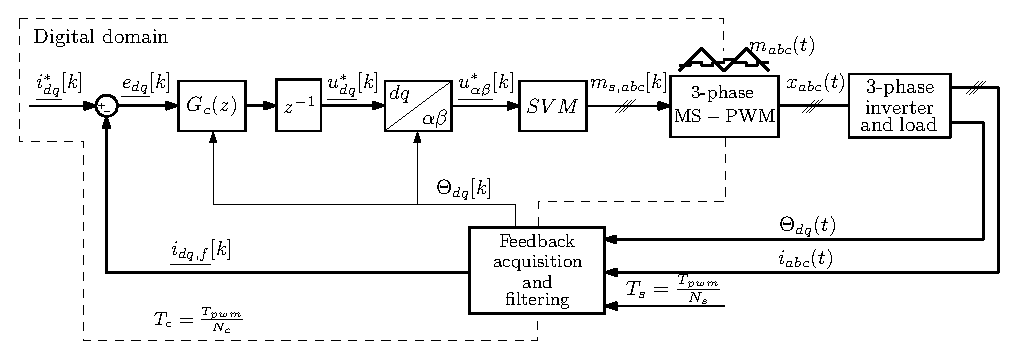
\includegraphics[width=0.8\linewidth]{figures/schematic.eps}}
    \caption{Multisampled control loop of a three-phase current-controlled inverter. The feedback acquisition and filtering is explained in subsection III A.}
    \label{fig:MSControl}
\end{figure*}

The multi-rate control system of a three-phase $RL$ load in $dq$ frame is shown in Fig. 1. The system can be separated into digital and continuous-time domain. An ADC is used to transform feedback signal from analog to digital domain. This action is performed with a sampling frequency $f_s = N_s f_{pwm}$, where $N_s$ is the multisampling (oversampling) factor and $f_{pwm}$ is the switching frequency of the inverter. The digital domain operates with frequency $f_c = N_c f_{pwm}$, where $N_c$ is the multi-update factor that determines the update rate of the controller output. The choice of this frequency is independent of the sampling frequency, as the feedback signal can be oversampled with frequency $f_s$ and then filtered and decimated to control frequency $f_c$. The digital domain is comprised of feedback filter $G_{fb}(z)$, controller $G_c(z)$, coordinate frame transformation block, and transformation from the reference voltage in $\alpha \beta$ frame to modulating waveforms in $abc$ frame. The controller $G_c(z)$ outputs reference voltage in $dq$ frame, $\underline{u_{dq}}^*[k]$, which is then transformed to $\alpha \beta$ frame. This reference voltage is used to obtain digital modulating waveform for each inverter phase, $m_{s,abc}[k]$. Conversion from digital to analog domain is performed by MS-PWM. Its inherent zero-order hold function transforms the digital impulse train $m_{s,abc}[k]$ into the continuous-time modulating waveform $m_{abc}(t)$. MS-PWM with the triangular carrier is used due to its favorable characteristics in MS-MU-PWM control \cite{corradini2018}. The PWM output is used as a gate signal $x_{abc}(t)$. The three-phase inverter is used to supply a generic $RL$ load, which can model either an AC electrical machine or the electrical grid. The sensed feedback includes line currents $i_{abc}(t)$ and the angle of the $dq$ coordinate frame $\Theta_{dq}$. 

\subsection{Motivation behind MS-MU-PWM control}

Modern processors feature high computational power, which enables short execution times for control routines. However, switching frequencies of power converters are hardware limited, and do not go over several tens of kHz for medium power applications. This hardware based limitation directly affects the realizable bandwidths of the current control loop, which subsequently limits the outer control loops. Therefore, pushing for highest possible bandwidths relative to the switching frequency is often a design criterion. One way of achieving that is the implementation of MS-MU-PWM.

Using describing function approach, small-signal model of the multisampled PWM with triangular carrier is found to be almost equal to a pure delay of $\frac{T_c}{2}$, where $T_c$ is the modulating waveform update period \cite{corradini2018}, i.e:

\begin{equation}
\begin{aligned}
G_{DPWM} (s) = \frac{d(s)}{m(s)} = A(\omega,D,N_c) e^{-s\frac{T_c}{2}},
\label{eq:DPWM} 
\end{aligned}    
\end{equation}
where $s$ is the complex variable of the Laplace transform, $d$ is the continuous-time duty cycle used for averaged modeling, $\omega$ is the angular frequency, and $D$ is the steady-state duty cycle. The gain $A$ can be approximated with unity gain with negligible losses in modeling accuracy \cite{corradini2018}.
In DSP applications, update of the modulating waveform is usually delayed by one control period $T_c$, due to the non-negligible computational time \cite{Buso2015}. This update delay can be represented in s-domain as:

\begin{equation}
\begin{aligned}
G_{ud} (s) = e^{-sT_c}.
\label{eq:updateDelay} 
\end{aligned} 
\end{equation}

Combining delays due to modulation \eqref{eq:DPWM} and algorithm computation \eqref{eq:updateDelay} results in total digital delay being equal to:

\begin{equation}
\begin{aligned}
\tau_{d} = \frac{3}{2}T_c = \frac{3}{2} \frac{T_{pwm}}{N_c}.
\label{eq:tauD} 
\end{aligned}    
\end{equation}

From \eqref{eq:tauD}, it can be seen that multi-update control reduces digital delays inversely to the multi-update factor $N_c$. Traditionally, double-update is the most often used method, which results in twice decreased delays compared to single-update.
The term multisampled (multi-update) control is most often used when $N_c$ is increased above 2. This kind of control is a promising way of bringing the digital control close to analog regarding achievable bandwidths. However, care must be taken as significant nonlinearities are also introduced in the control system, mainly due to the discontinuity of the modulating waveform, which now features switching ripple components as well. For this reason, multi-update control is most often followed by feedback filtering, which entirely removes the switching ripple from the feedback signal. Note that the discontinuity problems are strongly suppressed at high values of multi-update rate \cite{corradini2018}.

\subsection{Discrete-time model of a three-phase RL load}

Given the simplicity of the inverter topology with a $RL$ load, its model can be easily derived directly in discrete-time domain, which is suitable for the design of digital controllers. Note that for direct-discrete modeling, the action of the PWM is assumed to be equal to a zero-order hold in stationary $\alpha \beta$ frame:
\begin{equation}
\begin{aligned}
G_{DPWM,\alpha \beta} \approx \frac{1-e^{-sT_c}}{s}.
\label{eq:DPWMAlphaBeta} 
\end{aligned}    
\end{equation}
While the exact model is shown in \eqref{eq:DPWM}, for the very specific case of triangular carrier, MS-PWM can still be well-approximated with a ZOH with the update rate equal to $f_c$.

The direct discrete-time modeling can be found in ~\cite{lorenz2010,vuksa2016,commentsHoffmann}. This paper follows the procedure from \cite{commentsHoffmann}.
In order to analyze the three-phase $RL$ load as single-input single-output (SISO) system, complex variables are used. 
Starting from the $\alpha \beta$ frame, the differential equations necessary for modeling are:

\begin{equation}
\begin{aligned}
\underline{u}_{\alpha \beta} (t) = R \underline{i}_{\alpha \beta} (t) + L \frac{d}{dt} \underline{i}_{\alpha \beta} (t),
\label{eq:alphaBetaVoltage} 
\end{aligned}    
\end{equation}
where $R$ and $L$ are the line resistance and the line inductance, respectively. The machine back-emf or the grid voltage is neglected in this analysis, as the paper does not take into account the disturbance rejection.
The s-domain transfer function from applied voltage to the line current, corresponding to \eqref{eq:alphaBetaVoltage} is:

\begin{equation}
\begin{aligned}
G_{i,\alpha \beta} = \frac{1}{R} \frac{1}{1 + s \frac{L}{R}}.
\label{eq:sDomainAlphaBeta} 
\end{aligned}    
\end{equation}

Multiplication of \eqref{eq:updateDelay}, \eqref{eq:DPWMAlphaBeta} and \eqref{eq:sDomainAlphaBeta} yields the plant model in $\alpha \beta$ frame.
The transformation from $\alpha \beta$ to $dq$ frame is obtained using the substitution $s \rightarrow s + j \omega_o$, where $\omega_o$ is the $dq$ frame rotating frequency.
This yields the following s-domain plant transfer function in $dq$ frame:

\begin{equation}
\begin{aligned}
G_{p,dq}(s) = e^{-(s+j\omega_o) T_c} \frac{1-e^{-(s+j\omega_o) T_c}}{s+j\omega_o} \frac{1}{R} \frac{1}{1 + s \frac{L}{R} + j\omega_o \frac{L}{R}}.
\label{eq:modelSdomain} 
\end{aligned}    
\end{equation}
 
The discrete-time model is obtained directly from \eqref{eq:modelSdomain} using $\mathcal{Z}$ transform table:

\begin{equation}
\begin{aligned}
G_{p,dq}(z) = \frac{\left( 1 - e^{-\frac{R}{L}T_c}\right) e^{-2j\omega_o T_c}}{R} \frac{1}{z \left( z - e^{- \left( \frac{R}{L} + j\omega_o\right) T_c}\right)},
\label{eq:modelZdomain} 
\end{aligned}    
\end{equation}
where $z$ is the complex variable of the $\mathcal{Z}$ transform.

The model obtained in \eqref{eq:modelZdomain} is used for the subsequent derivation of the model-based controller.
 
\subsection{Discrete IMC controller}


\begin{figure}[t!]
    \centerline{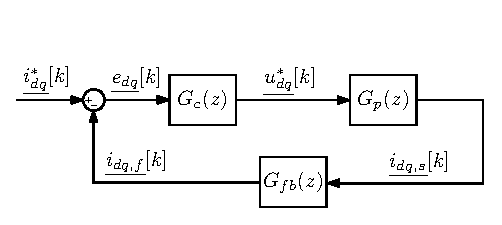
\includegraphics[width=0.95\linewidth]{figures/small_signal.eps}}
    \caption{Small-signal block diagram of the system from Fig. \ref{fig:MSControl} in discrete-time domain.}
    \label{fig:SmallSignal}
\end{figure}

The $dq$ frame discrete-time small signal block diagram of the control system in Fig. \ref{fig:MSControl} is shown in Fig. \ref{fig:SmallSignal}. The IMC controller is derived by inverting the plant model and adding an integrator with gain $\alpha$ that determines the crossover frequency \cite{vuksa2016}. For the sake of causality, due to digital delays, additional factor of $\frac{1}{z^2}$ is added to the controller structure, which results in the following transfer function:

\begin{equation}
\begin{aligned}
& G_{c}(z) =  \frac{\alpha \cdot z}{z-1} \frac{1}{z^2} G^{-1}_{p,dq}(z)  = \\
& =  \frac{\alpha \cdot R \cdot e^{j\omega_o T_c}}{\left( 1 - e^{-\frac{R}{L}T_c}\right)}\frac{z e^{j\omega_o T_c}-e^{-\frac{R}{L}T_c}}{z-1}.
\label{eq:Controller} 
\end{aligned}    
\end{equation}

By implementing the controller from \eqref{eq:Controller} without any feedback filters, the following open-loop transfer function is obtained:

\begin{equation}
\begin{aligned}
W_{ol,1}(z) = G_c(z) G_p(z) =  \frac{\alpha}{z(z-1)}.
\label{eq:OpenLoop} 
\end{aligned}    
\end{equation}

In \cite{vuksa2016} it is shown that relying on two samples per $T_{pwm}$ often results in unacceptable feedback signal deterioration in industrial applications. This is due to the unalignement between the voltage impulse and sampling instants due to limited current sensor bandwidths, analog feedback filters, delays in driver circuits, and similar. Furthermore, the feedback signal often comprises oscillations due to the $LC$ parasitics of long cables that are present in industrial drives. This is a motivation behind the implementation of MS-DU-PWM in \cite{vuksa2016} and MS-MU-PWM in this paper, where the signal is highly oversampled and then averaged over the switching period.

\section{Feedback acquisition, coordinate frame transformation, and filtering}

\subsection{Feedback acquisition and $\alpha \beta - dq$ transformation}

The timing diagram of feedback acquisition, coordinate frame transformation and controller update is shown in Fig. \ref{fig:timings}. The modulating waveform is illustrated for one phase, $m_a(t)$. Without the loss of generality, the transformation of line currents from $abc$ frame to $\alpha \beta$ frame is not shown in Fig. \ref{fig:timings}.
The digital system analyzed in this paper features two independent frequencies. First one is the control frequency, which defines the controller execution rate and update of the modulating waveform. It is defined by the multi-update factor $N_c$. Control interrupts over the switching period are synchronized with the carrier $w(t)$ such that the first one occurs when the carrier is equal to $0$ while other $N_c-1$ are delayed by $T_c$ each. 
The second frequency is the sampling frequency, which is defined by the multisampling factor $N_s$. This allows the DSP to acquire the signal with much higher rate than it can calculate the control algorithm, by employing the standardly available DMA module. High sampling rates allow the use of digital filters, for example MAFs, and subsequent decimation to provide the feedback $\underline{i_{dq,f}}[k]$ at the control execution rate.
Again, sampling instants are synchronized with the carrier such that the first one occurs when the carrier is equal to $0$. 

Fig. \ref{fig:timings} is given for $N_c = 4$ and $N_s = 16$. At instant $kT_c$, $dq$ frame feedback current $\underline{i_{dq,f}}[k]$ is obtained and used to calculate the voltage reference $\underline{u^*_{dq}}[k]$, which is used to calculate the segment of the modulating waveform that is applied at the beginning of the following control interrupt. The synchronous frame angle $\Theta_{dq}$ is obtained each $T_c$ by implementing a PLL or using resolver/encoder sensors. 

\begin{figure}[t!]
    \centerline{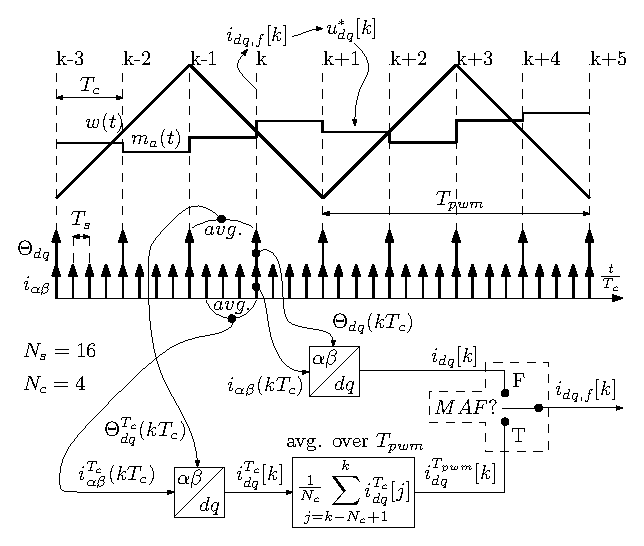
\includegraphics[width=0.95\linewidth]{figures/timing_diagram.eps}}
    \caption{Timing illustration for signal acquisition, filtering, and modulating waveform update. The position of the selector $MAF?$ determines whether the feedback currents are obtained without filtering or using one switching period averaging. The figure is given for $N_s = 16$ and $N_c = 4$.}
    \label{fig:timings}
\end{figure}

As shown in Fig. \ref{fig:timings}, the selector $MAF?$ chooses whether the feedback is provided without any filtering, or using a MAF over the switching period. In the first case, the latest samples of $\underline{i_{\alpha \beta}}(kT_c)$ and $\Theta_{dq}(kT_c)$ are used to obtain the $dq$ frame current $\underline{i_{dq}}[k]$, which is used as the feedback signal. In case when $N_c = N_s = 2$, we obtain the standardly used DS-DU control. In cases when $N_c = N_s > 2$, we obtain the MS-MU-PWM with switching ripple in the feedback signal \cite{Petric2020}.

In cases when the MAF is used, the goal is to obtain a true average value of $dq$ currents over one switching period. The $\alpha \beta$ currents are first averaged over $T_c$, using $\frac{N_s}{N_c}$ latest current samples, to obtain $\underline{i_{\alpha \beta}}^{T_c} (kT_c)$. This average current is then transformed to $dq$ frame to obtain $\underline{i_{dq}}^{T_c} [k]$. The transformation is performed using the angle $\Theta_{dq}^{T_c}(kT_c)$, calculated as an average of two latest angle values. If $N_c\geq 2$, currents are further averaged using $N_c$ values of $\underline{i_{dq}}^{T_c}$ to obtain the average value during the previous switching period $\underline{i_{dq}}^{T_{pwm}}[k]$.
For this filtering strategy, in cases when $N_s>N_c = 2$, we obtain MS-DU control, where the filtering is used to obtain a true-average value at the expense of reduced system dynamics \cite{vuksa2016}. In cases when $N_s \geq N_c > 2$, we obtain MS-MU-PWM control with switching ripple being filtered from the feedback signal. The factor $N_s$ is chosen to be as high as allowed by the maximum ADC sampling rate.
Note that independently of whether the MAF is used or not, transformation of the reference voltage from $dq$ to $\alpha \beta$ frame, shown in Fig. \ref{fig:MSControl}, is always performed with the latest value of the angle $\Theta_{dq}(kT_c)$.

\subsection{Total time delay in DSP applications}

For control loop analysis and comparison between DS-DU-PWM, MS-DU-PWM, and MS-MU-PWM based on the crossover frequency and phase margin it is of interest to analyze the loop delays in continuous-time domain.

The equivalent time delay of the algorithm calculation and the DPWM modulation is shown in \eqref{eq:tauD}. For DS-DU-PWM without any feedback filtering, this corresponds to the total delay:

\begin{equation}
\begin{aligned}
\tau_{d,DS-DU} = \frac{3}{2} \frac{T_{pwm}}{2}.
\label{eq:tauDSDU} 
\end{aligned}    
\end{equation}

For MS-DU-PWM, the MAF is most often used to filter out the switching frequency component. The phase lag of the MAF over $T_{pwm}$ can be closely approximated by a pure delay equal to $\frac{T_{pwm}}{2}$. This results in the equivalent time-delay:

\begin{equation}
\begin{aligned}
\tau_{d,MS-DU,MAF} = \frac{3}{2} \frac{T_{pwm}}{2} + \frac{T_{pwm}}{2} = \frac{5}{4} T_{pwm}.
\label{eq:tauMSDU} 
\end{aligned}    
\end{equation}

For MS-MU-PWM without MAF, equivalent time-delay is equal to \eqref{eq:tauD}.
Finally, for MS-MU-PWM with MAF, equivalent time-delay is:
\begin{equation}
\begin{aligned}
\tau_{d,MS-MU,MAF} = \frac{3}{2} \frac{T_{pwm}}{N_c} + \frac{T_{pwm}}{2} = \frac{\frac{3}{N_c}+1}{2}T_{pwm}.
\label{eq:tauMSMUMAF} 
\end{aligned}    
\end{equation}

The MS-DU-PWM features significant time-delay due to MAF and high modulating and control delays. For high dynamic performance, MS-DU-PWM controller structure needs to include additional derivative gain compared to \eqref{eq:Controller}, to compensate for the high delays \cite{vuksa2016}. Regarding dynamics, best case is represented by the MS-MU-PWM without MAF. For multi-update factors $N_c \geq 8$, control delays are practically removed and dynamic capabilities become equal to the ones of analog controllers.
Finally, from \eqref{eq:tauMSMUMAF} it can be seen that for MS-MU-PWM with a MAF, starting from $N_c>6$, equivalent time delay is lower than for the DS-DU-PWM. This is important as it states that the same kind of filtering as in MS-DU-PWM can be used to obtain a high quality feedback signal while improving dynamics, instead of deteriorating it, compared to standardly used DS-DU-PWM.

\section{Controller parameter design}
For the purpose of controller tuning, the analysis is performed in discrete-time domain, with a rate equal to $f_c$. For this purpose, even if $N_s > N_c$, the MAF is approximated as a filter at frequency $f_c$ using the following transfer function \cite{vuksa2016}:

\begin{equation}
\begin{aligned}
G_{MAF}(z) = \frac{1 + 2z^{-\frac{N_c}{2}} + z^{-N_c}}{4}.
\label{eq:MAF} 
\end{aligned}    
\end{equation}

For the tested methods that do not use the feedback filter, the open-loop transfer function is given in \eqref{eq:OpenLoop}. For methods that use the MAF, the open loop transfer function is equal to:

\begin{equation}
\begin{aligned}
W_{ol,2}(z) = W_{ol,1}(z) G_{MAF}(z)
\label{eq:OpenLoop_MAF} 
\end{aligned}    
\end{equation}

For a clear dynamic comparison, the controller gain $\alpha$ in \eqref{eq:Controller} is set such that the phase margin equal to $70^o$ is achieved for all tested methods. In this way, the crossover frequency is increased for methods with a lower equivalent time delay. 
In this paper, the verification is performed on a BLDC motor, with parameters shown in Table \ref{tab:motor_param}:

\begin{table}[h!]
			  \caption{Machine and Inverter Parameters}
              \label{tab:motor_param}
              \centering
              \begin{tabular}{llll}
                           \midrule\midrule
        BLDC motor & label & value   & unit\\
        \midrule               
                  Number of poles	& $2p$ & 6 & /\\
                  Rated torque  & $T_{nom}$ & 6 &  $\mathrm{Nm}$  \\
                  Rated current  & $I_{nom}$ & 7.3 &  $\mathrm{A_{rms}}$  \\
                  Torque constant  & $k_{t}$ & 0.821 & $\mathrm{Nm/(A_{rms})}$   \\
                  Back-EMF constant  & $k_{e}$ & 1.2534 & $\mathrm{V_{peak}/(rad/s)}$   \\
                  Stator resistance  & $R_{s}$ & 0.47 & $\mathrm{\Omega}$   \\
                  Stator inductance  & $L_{s}$ & 3.4 & mH   \\
                  \midrule\midrule

        Inverter & label & value   & unit\\
        \midrule               
                  DC link voltage	& $V_{dc}$ & 520 & V \\  
                  Switching frequency  & $f_{pwm}$ & 10 & kHz   \\
                  Dead time  & $t_{dt}$ & 1 &  $\mathrm{\mu s}$  \\
                  \midrule\midrule
                                                        
              \end{tabular}
\end{table}


The first tested strategy is the standardly used DS-DU approach. For a $70^o$ phase margin, the value of $\alpha$ is equal to $0.23$ and the achieved crossover frequency is equal to $7.3 \% f_{pwm}$.
The second tested strategy is the MS-DU control with the oversampled MAF in the feedback path. The controller gain $\alpha$ is equal to $0.14$, which sets the crossover frequency to $4.4 \% f_{pwm}$.
Finally, the gain $\alpha$ of the proposed MS-MU method with a MAF based feedback acquisition is equal to $0.0636$, which sets the crossover frequency to $8 \%  f_{pwm}$. The MS-MU-PWM without ripple filtering is not implemented, as the modulating waveform discontinuity impact in three-phase applications is still not properly investigated\footnote{Modulating waveform discontinuities may result in reduced-, zero-, or infinite-gain zones in the modulator transcharacteristic. The impact of these zones is analyzed in \cite{corradini2018} and \cite{Petric2021}. Quantification of resulting nonlinearities and conditions for their appearance in single-phase systems is being investigated by the authors. For three-phase systems without a neutral wire, the switching ripple is coupled between the phases, which is why a separate analysis is required.}. 
For both MS-DU and MS-MU, the multisampling ratio is set to $N_s = 16$. For MS-MU, the multi-update ratio is chosen as $N_c = 8$, which was limited by the algorithm execution time on the used DSP.
The closed-loop $-3$ dB bandwidth is calculated using $W_{cl,1}(z) = \frac{W_{ol,1}(z)}{1+W_{ol,1}(z)}$ for the case of DS-DU and $W_{cl,2}(z) = \frac{G_c(z) G_p(z)}{1+W_{ol,2}(z)}$ for the case of MS-DU and MS-MU. The summary of control loop parameters are shown in Table \ref{tab:an_param}. It can be seen that the MS-MU with the MAF achieves better dynamics than the DS-DU.

\begin{table}[h!]
			  \caption{Control loop parameters}
              \label{tab:an_param}
              \centering
              \begin{tabular}{llll}
                           \midrule\midrule
        DS-DU & label & value   & unit\\
        \midrule               
                  IMC gain	& $\alpha$ & 0.23 & /\\  
                  Cross-over frequency  & $f_{c}$ & 735 & Hz   \\
                  Phase margin  & $pm$ & 70.2 &  $^\circ$  \\
                  Closed-loop bandwidth  & $f_{bw}$ & 1253 & Hz   \\
                  \midrule\midrule

        MS-DU with MAF, $N_s = 16$ & label & value   & unit\\
        \midrule               
                  IMC gain	& $\alpha$ & 0.14 & /\\  
                  Cross-over frequency  & $f_{c}$ & 445 & Hz   \\
                  Phase margin  & $pm$ & 70 &  $^\circ$  \\
                  Closed-loop bandwidth  & $f_{bw}$ & 766 & Hz   \\
                  \midrule\midrule
      MS-MU with MAF, $N_s = 16$ , $N_c =  8$ & label & value   & unit\\
        \midrule               
                  IMC gain	& $\alpha$ & 0.0636 & /\\  
                  Cross-over frequency  & $f_{c}$ & 799 & Hz   \\
                  Phase margin  & $pm$ & 70.3 &  $^\circ$  \\
                  Closed-loop bandwidth  & $f_{bw}$ & 1387 & kHz   \\
                  \midrule\midrule
                                                        
              \end{tabular}
\end{table}

\subsection{Verification of discrete-time modelling}
For proposed MS-MU with MAF, simulations in MATLAB/Simulink were performed in order to verify the discrete-time modeling. 
The sweep frequency response analysis (SFRA) is performed to verify the open-loop transfer function \eqref{eq:OpenLoop_MAF} for parameters in Table \ref{tab:motor_param} and Table \ref{tab:an_param}. In simulations, a detailed model of the DPWM, which resembles the action qualifier module realization within the DSP TI f28379d EPWM peripheral, is implemented. The motor is modeled in the continuous-time domain using the Simulink $abc$ frame machine model. The motor speed is set to $565$ rpm, which results in the output frequency $f_o = 270$ Hz.
For the measured axis response, the perturbation magnitude is set to $0.1$ A, while for the other axis the controller input is set to $0$. The perturbation frequencies are an arithmetic sequence from $400$ Hz to $5000$ Hz, with a step of $230$ Hz. The $q-axis$ open loop SFRA result is shown in Fig. \ref{fig:MSMUmaf_olfra}. The simulated results are compared to the analytics and it can be seen that a very good match is achieved.

\begin{figure}[t!]
    \centerline{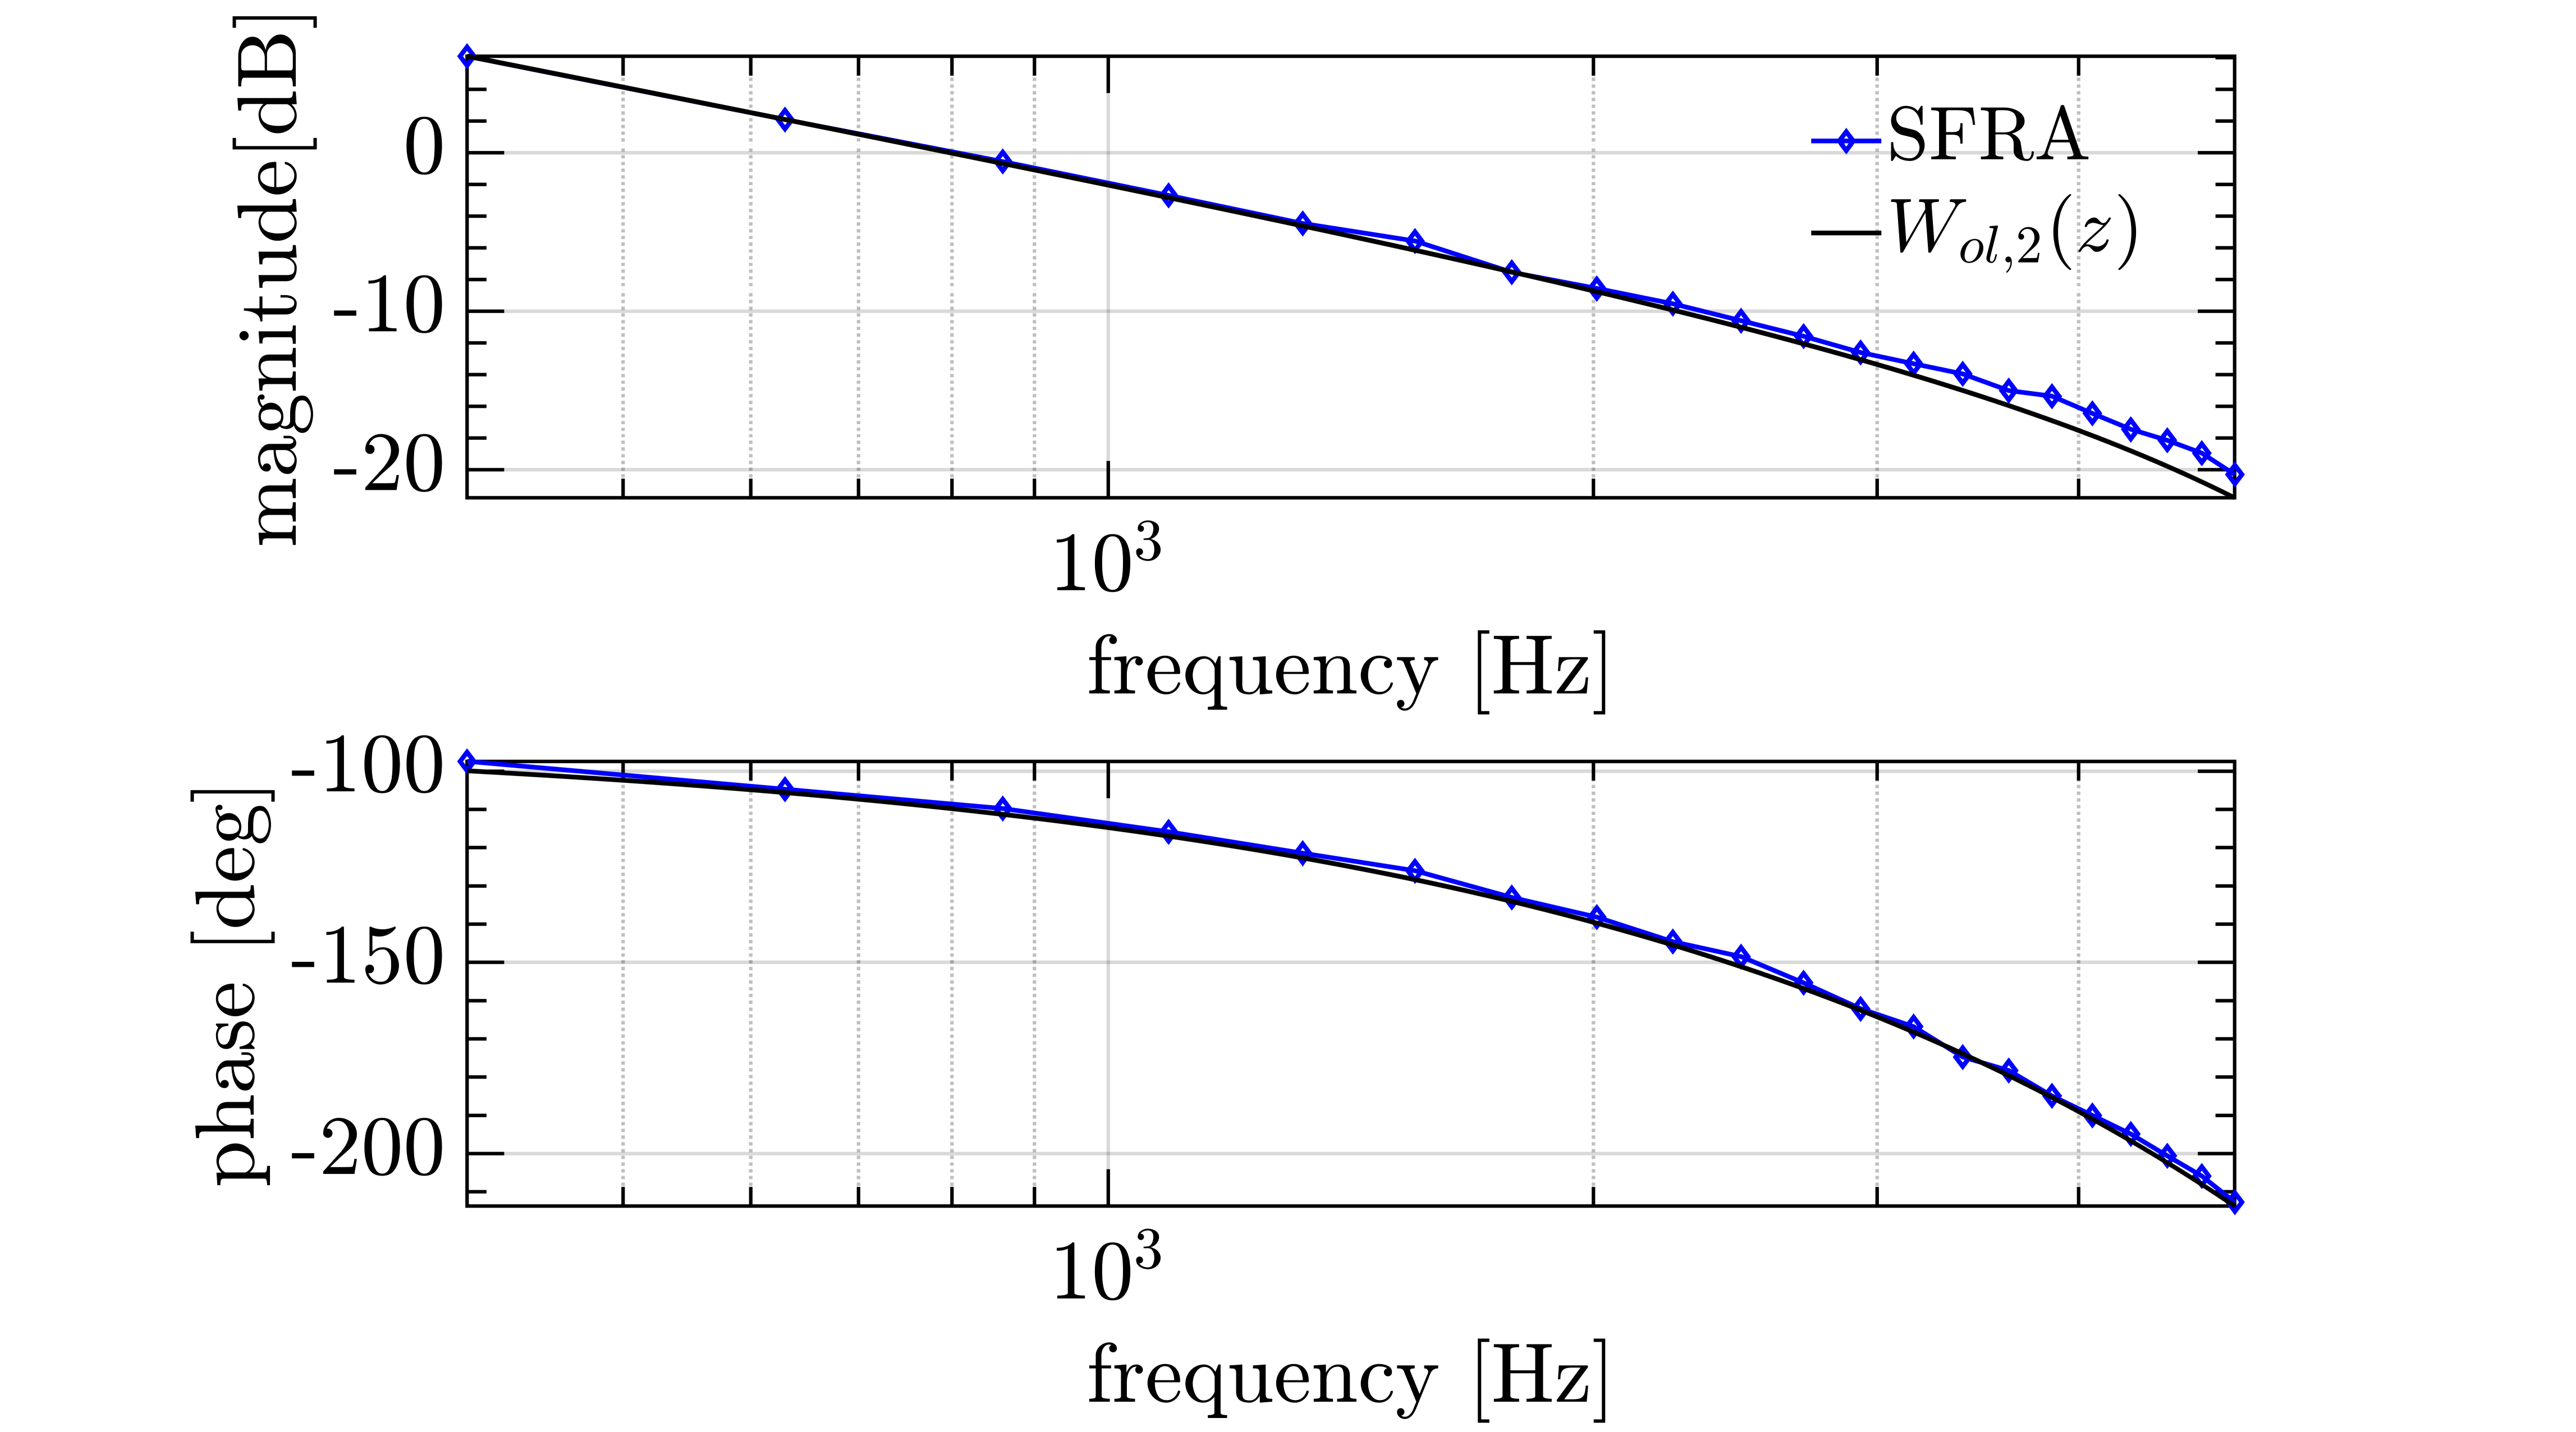
\includegraphics[width=1\linewidth]{figures/ivan figs/MSMU_OL_SFRA.png}}
    \caption{Simulated SFRA results for open-loop system with the MS-MU control strategy. The drive parameters are shown in Table \ref{tab:motor_param} and the controller parameters are shown in Table \ref{tab:an_param}. The results are compared with the analytic frequency response of $W_{ol,2}(z)$. }
    \label{fig:MSMUmaf_olfra} 
\end{figure}


\section{Experimental verification}
This section provides the experimental validation of the previously discussed controllers using the Typhoon HIL 402 platform and DSP TI f28379d. Power stage is implemented within hardware-in-the-loop (HIL) simulation model and comprises DC voltage source, IGBT inverter and BLDC motor with parameters from Table \ref{tab:motor_param}. The motor line currents are obtained via HIL’s analog outputs and are routed to DSP's ADC inputs. The motor angle information is obtained using the encoder signals, which are sent from HIL’s digital outputs to the DSP's QEP inputs. These current and position feedback signals are used to perform the FOC algorithm in the DSP in the same way as described in Section III. The resulting gate signals are sent from DSP’s EPWM outputs to HIL's digital inputs. 
Note that a particular logic had to be implemented in the DSP algorithm, in order to allow the implementation of MS-PWM without the occurrence of pulse-skipping. Namely, the used DSP from TI modifies the PWM output when the modulating waveform is strictly equal to the carrier's counter value. This prevents the detection of vertical crossings \cite{corradini2018}, which results in full or zero duty cycle. The situation comprising a vertical crossing is illustrated in Fig. \ref{fig:timings} at the instant $kT_c$.
The added logic prolongs the algorithm execution time, but still allows the complete $FOC$ algorithm to run at $N_c=8$ and $f_{pwm} = 10$ kHz.

For each of the control strategies analyzed in Section IV, HIL simulations were performed to obtain $q$-axis current step responses and compare them to the step response of the corresponding closed loop transfer functions $W_{cl,1}$ and $W_{cl,2}$. The motor speed is set to $565$ rpm, which results in the output frequency $f_o=270$ Hz. 
Step responses are shown in Figs. \ref{fig:DSDU_step}-\ref{fig:MSMUmaf_step}. Note that the presented HIL results are obtained by post-processing of the signals exported from DSP’s RAM. The line currents are acquired each $T_s$ and the angle is acquired each $T_c$. 
For visualization and comparison with the analytics, the switching ripple is removed using the same filtering approach as in Fig. \ref{fig:timings}, however in a non-causal manner so that delays are not added.
According to the presented results there is a very good match between experimental and analytical results for all compared control strategies. DC error which is visible in case of DS-DU controller (Fig. \ref{fig:DSDU_step}) is due to the aliasing mainly present as a consequence of the delay introduced by HIL (approximately $2.5$ us). This delay prevents the sampling instant to coincide with the middle of the current ripple. Note that this error can be partly compensated by offsetting the sampling instant, however, it was of interest to emphasize this drawback of the control methods that rely only on two samples per switching period. 

\begin{figure}[t!]
    \centerline{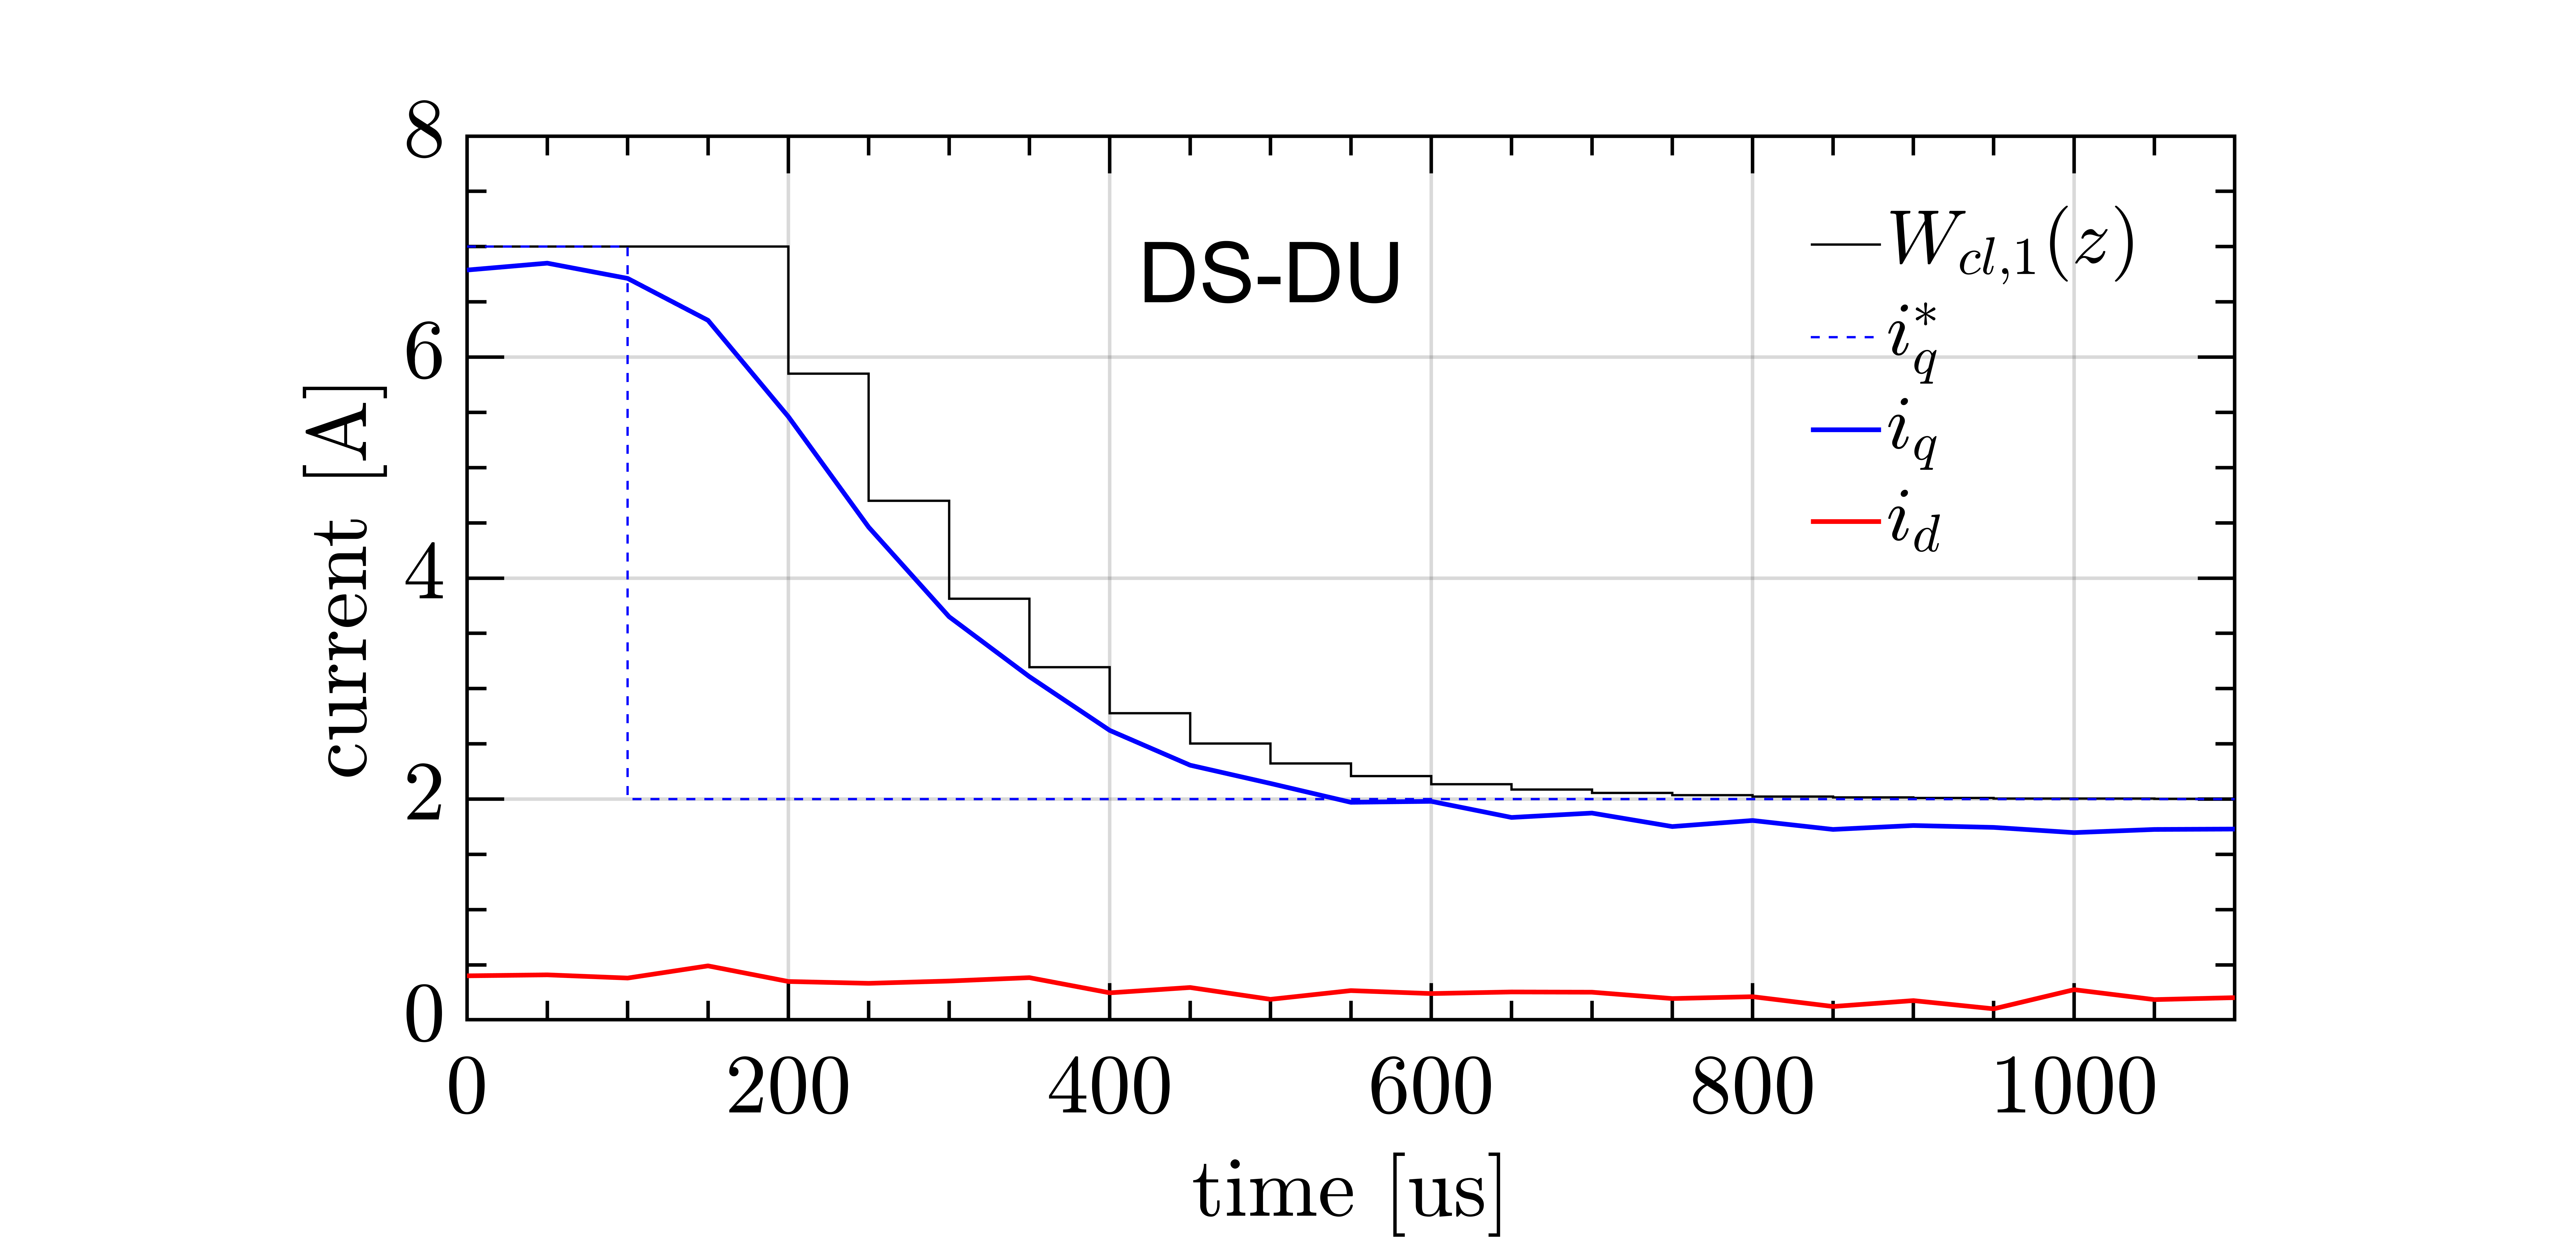
\includegraphics[width=1\linewidth]{figures/ivan figs/DSDUstepHIL.png}}
    \caption{Verification of a $q$-axis step response for DS-DU control strategy. The drive parameters are shown in Table \ref{tab:motor_param} and the controller parameters are shown in Table \ref{tab:an_param}. The results are compared with the analytical step response of $W_{cl,1}(z)$. The $d$-axis current is shown to demonstrate decoupling capabilities.}
    \label{fig:DSDU_step} 
\end{figure}
\begin{figure}[t!]
    \centerline{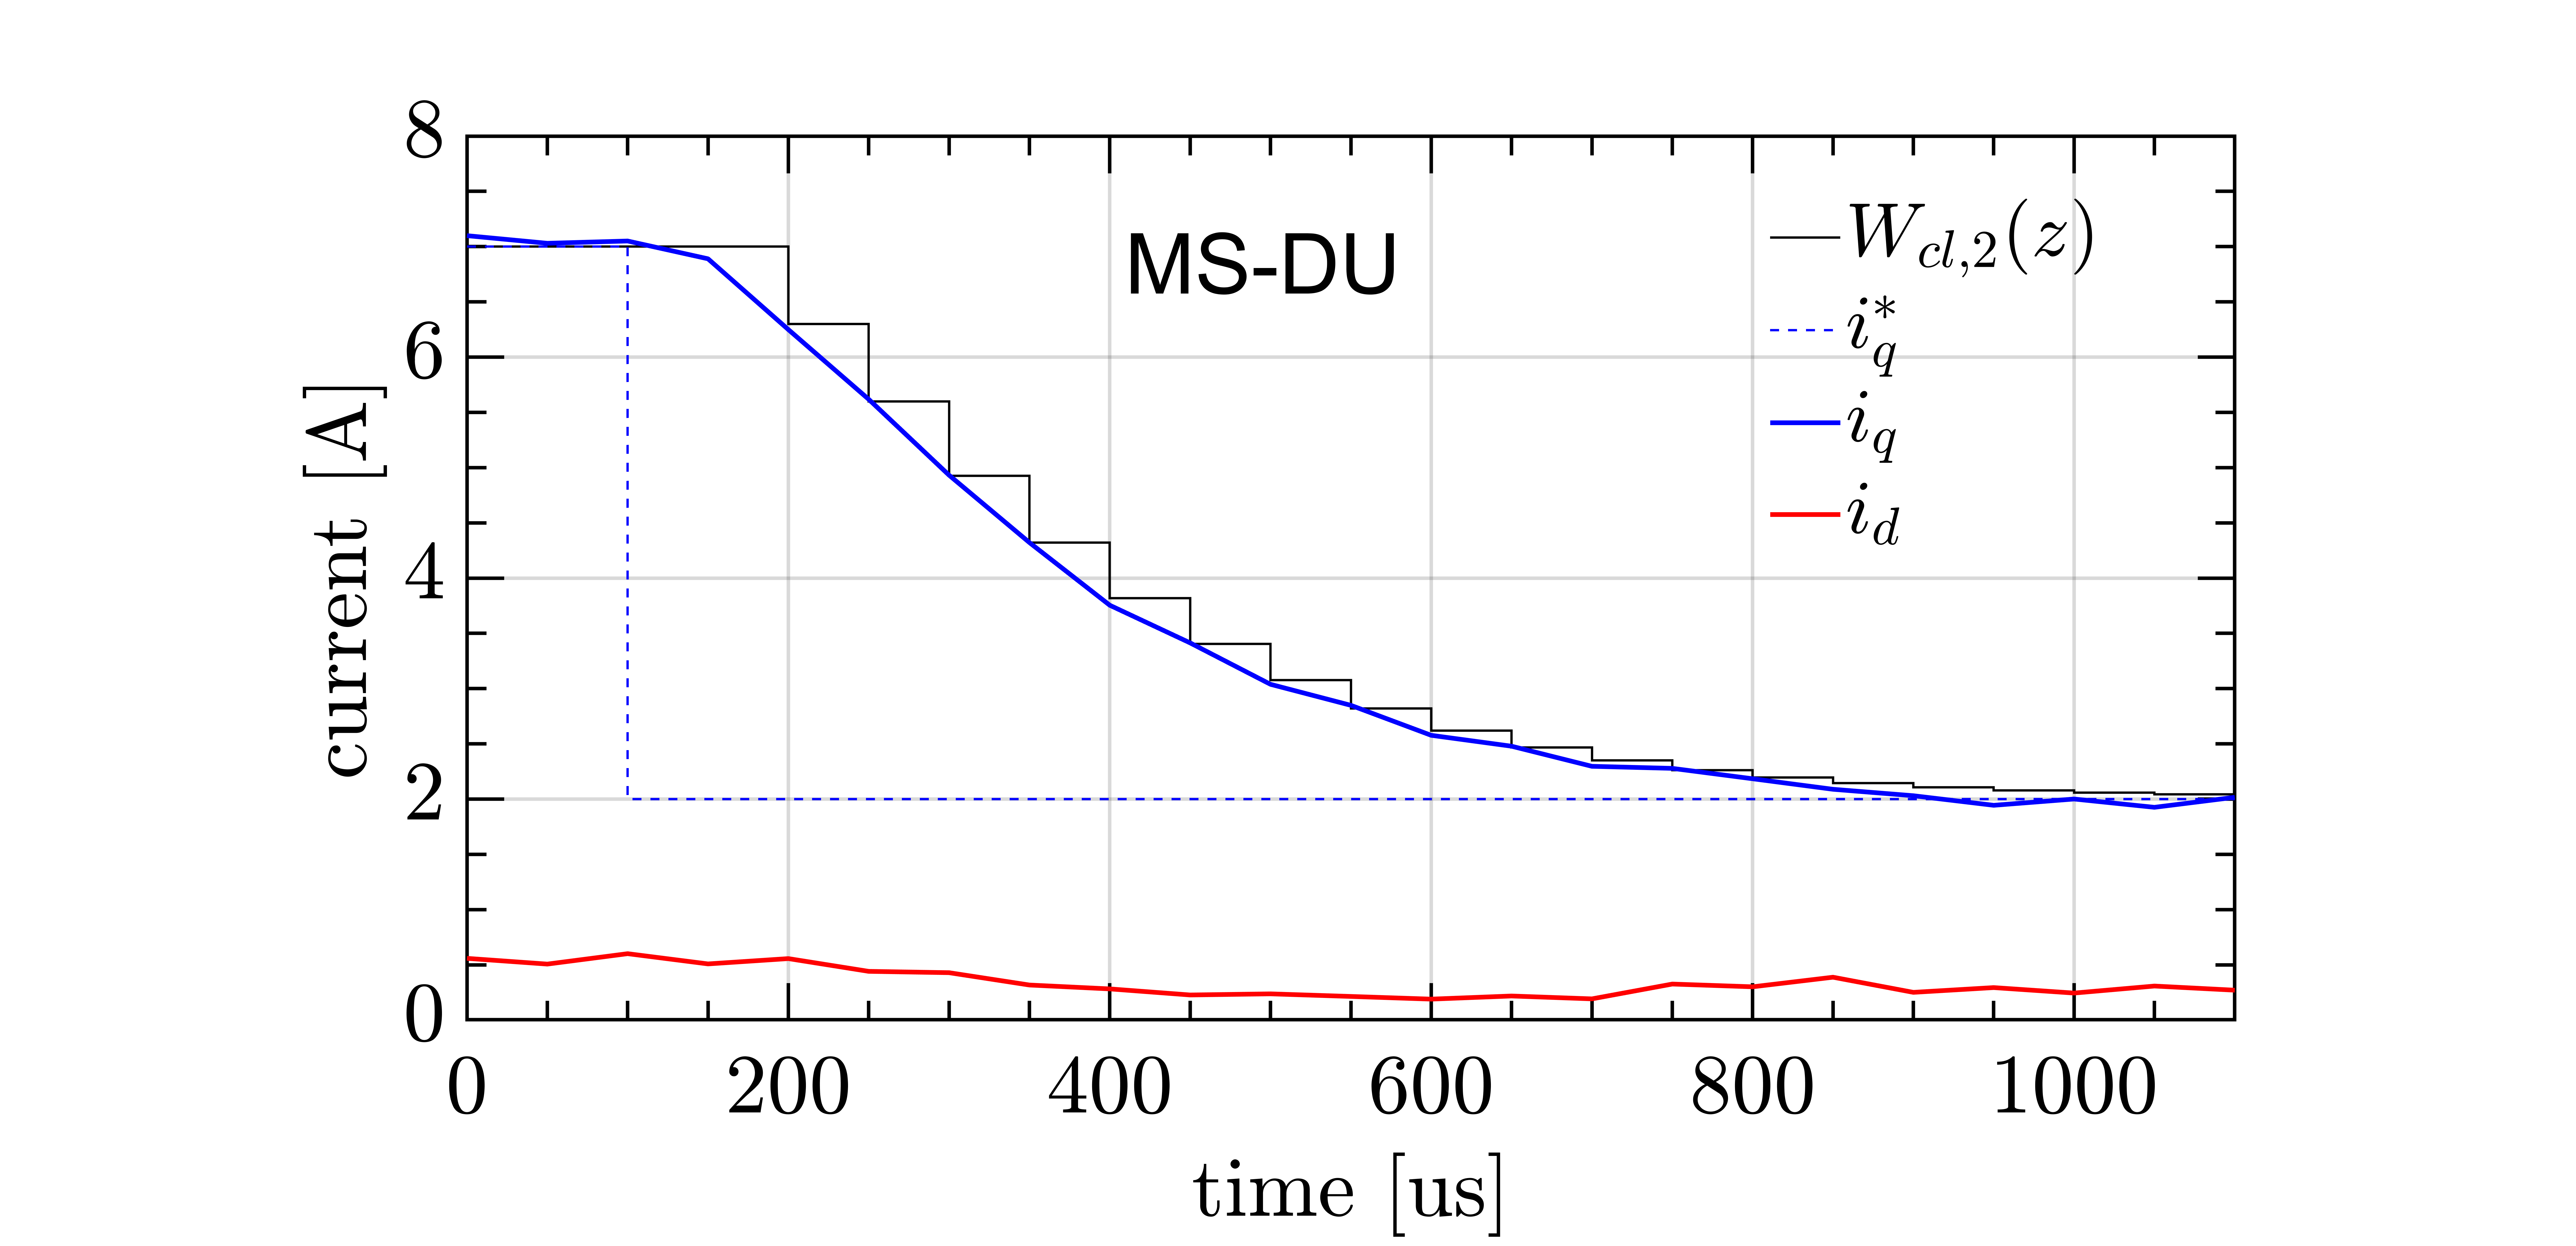
\includegraphics[width=1\linewidth]{figures/ivan figs/MSDUstepHIL.png}}
    \caption{Verification of a $q$-axis step response for MS-DU control strategy. The drive parameters are shown in Table \ref{tab:motor_param} and the controller parameters are shown in Table \ref{tab:an_param}. The results are compared with the analytical step response of $W_{cl,2}(z)$. The $d$-axis current is shown to demonstrate decoupling capabilities.}
    \label{fig:MSDU_step} 
\end{figure}
\begin{figure}[t!]
    \centerline{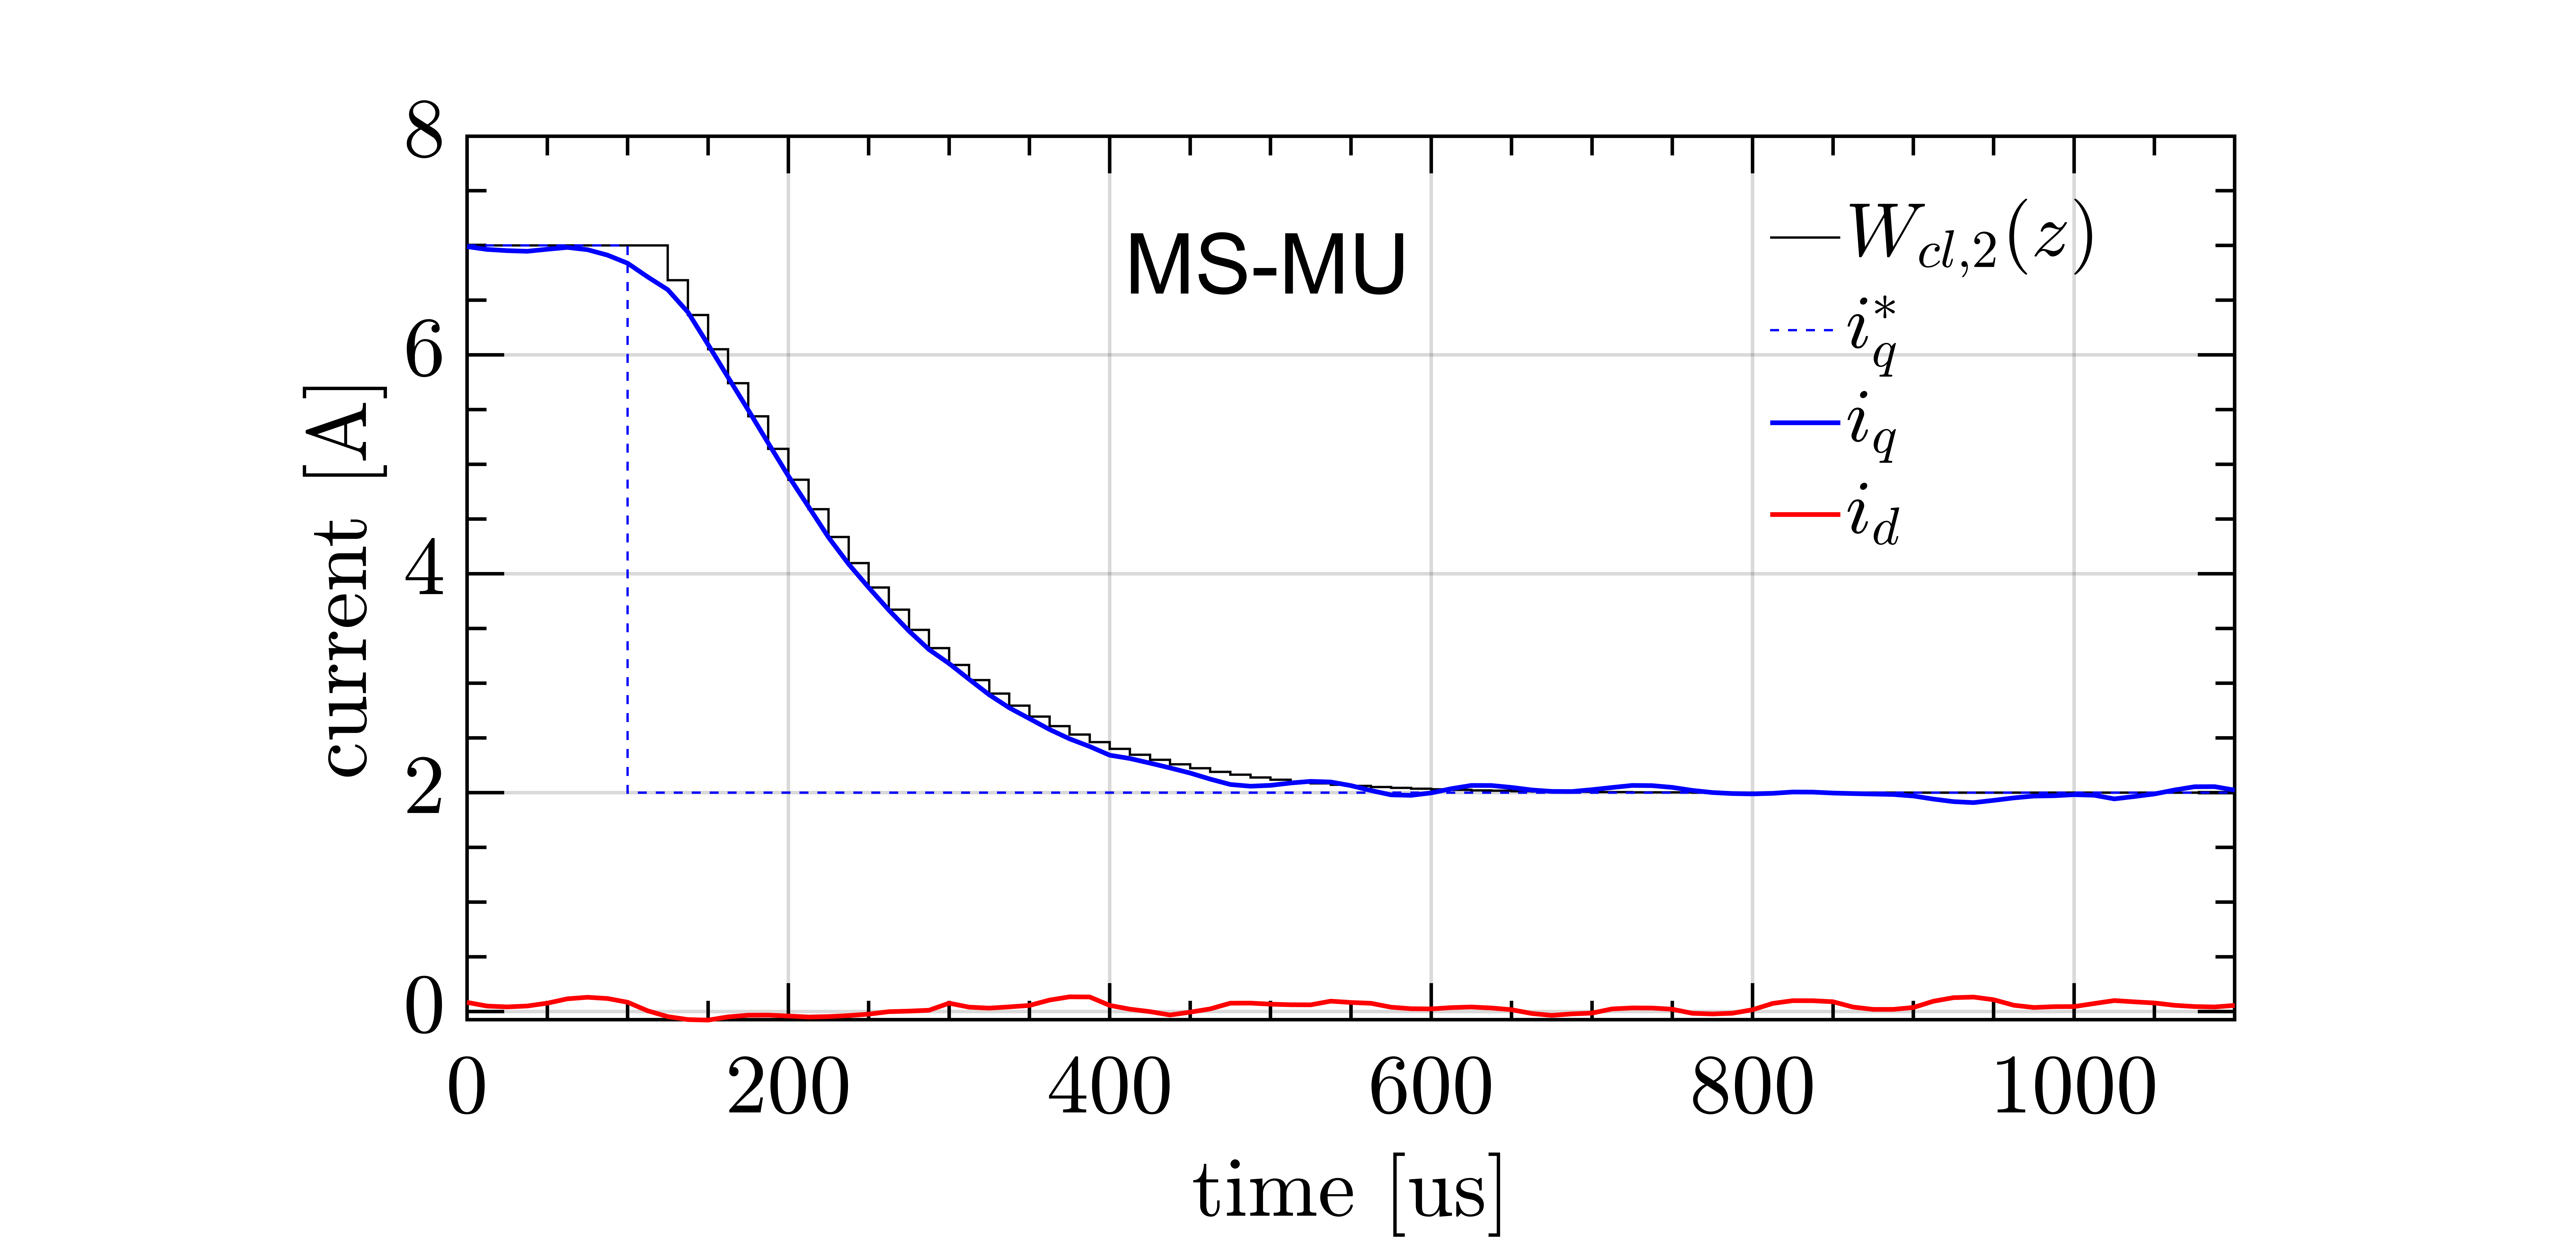
\includegraphics[width=1\linewidth]{figures/ivan figs/MSMUstepHIL.png}}
    \caption{Verification of a $q$-axis step response for MS-MU control strategy. The drive parameters are shown in Table \ref{tab:motor_param} and the controller parameters are shown in Table \ref{tab:an_param}. The results are compared with the analytical step response of $W_{cl,2}(z)$. The $d$-axis current is shown to demonstrate decoupling capabilities.}
    \label{fig:MSMUmaf_step} 
\end{figure}


\section{Conclusions}
This paper has presented a multisampled multi-update (MS-MU-PWM) current control strategy applied to a high-speed three-phase electric drive. The independent choice of sampling and control-update frequencies allows high-quality feedback acquisition with improved dynamic capabilities compared to the standard double-update method. The analysis is verified using a DSP TI f28379d and a Typhoon HIL 402 hardware-in-the-loop system.

\ifCLASSOPTIONcaptionsoff
  \newpage
\fi

\bibliographystyle{IEEEtran}
% argument is your BibTeX string definitions and bibliography database(s)
\bibliography{IEEEabrv,bib/mybibliography.bib}

\end{document}



